\tikzstyle{s} = [circle, minimum width=1cm, text width=1cm, minimum height=1cm, text centered, draw=black]
\tikzstyle{n} = [circle, minimum width=1cm, text width=1cm, minimum height=1cm, text centered, draw=black, fill=gray!30]
\tikzstyle{p} = [circle, minimum width=1cm, text width=1cm, minimum height=1cm, text centered, draw=black, line width=0.75mm, fill=gray!30]
\tikzstyle{arrow} = [thick,->,>=stealth]
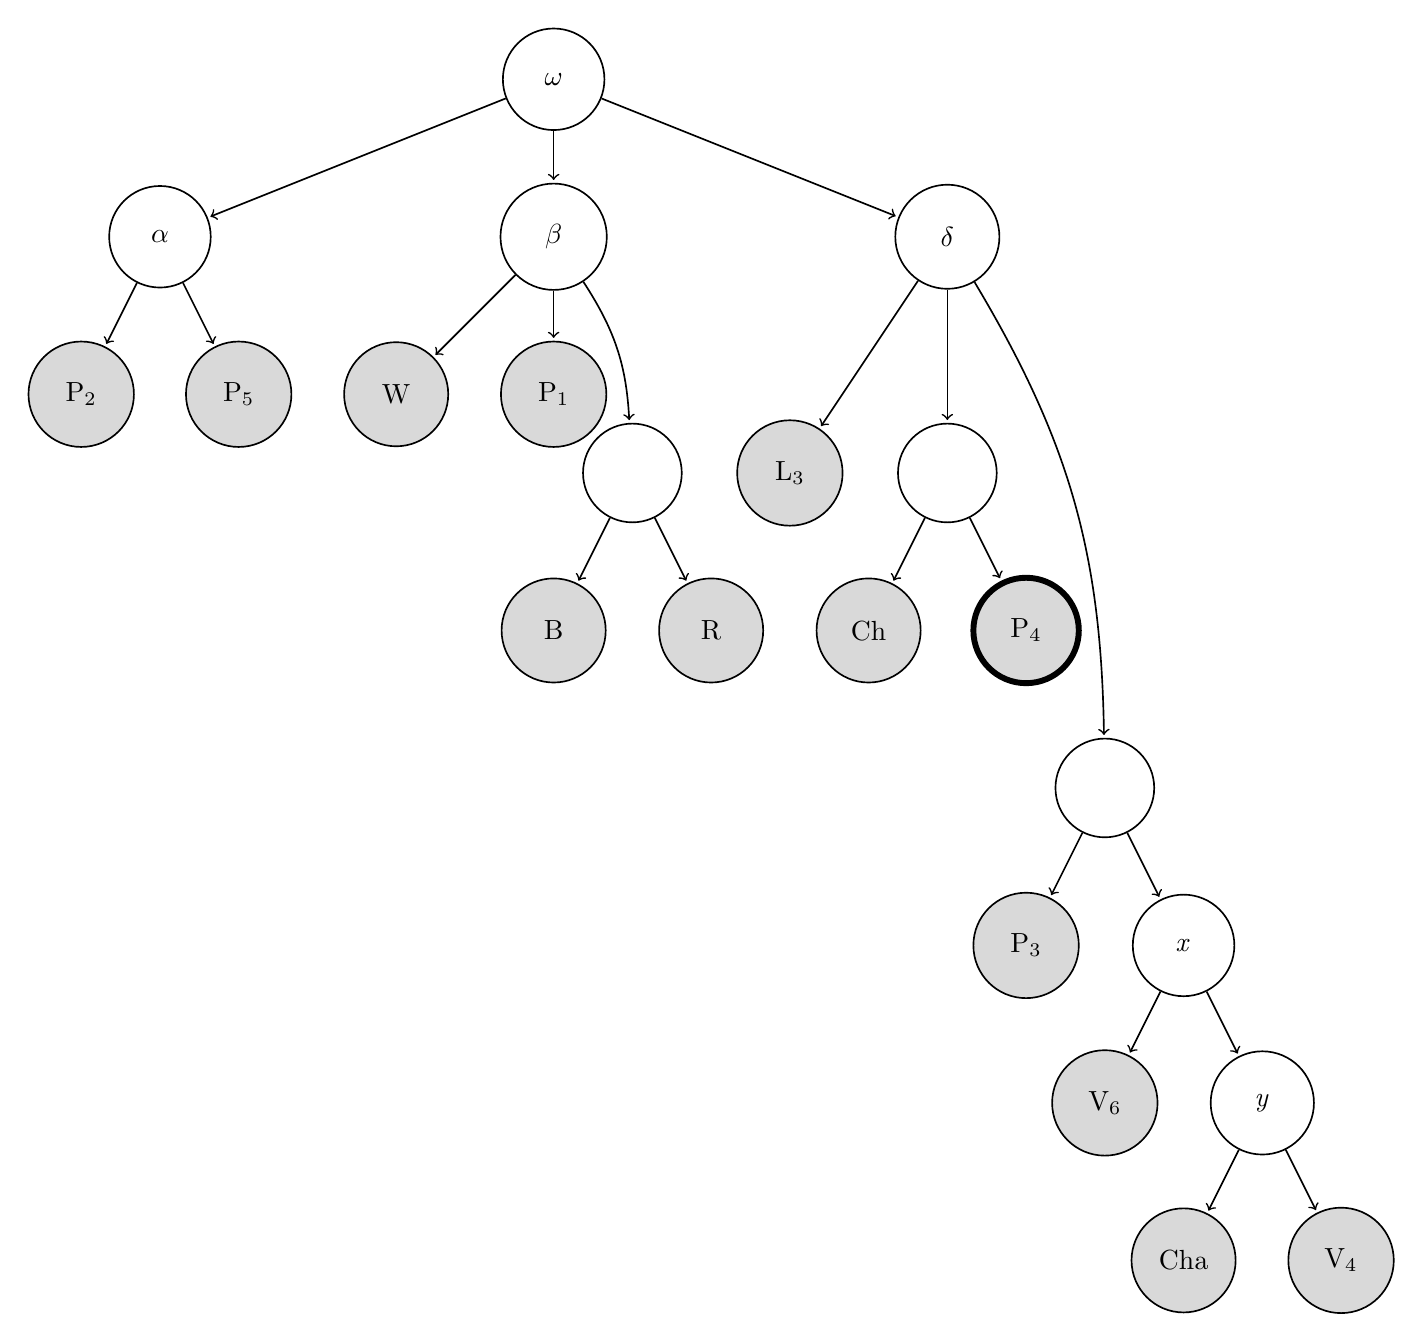
\begin{tikzpicture}[-,shorten >=1pt,auto,node distance=2cm,semithick]
\tikzstyle{every state}=[fill=red,draw=none,text=white]

\node[s] (w) {$\omega$};

\node[s] (a) [below of=w, xshift=-5cm] {$\alpha$};
\node[n] (p2) [below of=a, xshift=-1cm] {P\textsubscript{2}};
\node[n] (p5) [below of=a, xshift=1cm] {P\textsubscript{5}};

\path[every node/.style={font=\sffamily\small}]
    (w) edge[->] node[]{} (a)
    (a) edge[->] node[]{} (p2)
    (a) edge[->] node[]{} (p5)
;

\node[s] (b) [below of=w] {$\beta$};
\node[n] (W) [below of=b, xshift=-2cm] {W};
\node[n] (p1) [below of=b] {P\textsubscript{1}};
\node[s] (bb) [below of=b, yshift=-1cm, xshift=1cm] {};
\node[n] (B) [below of=bb, xshift=-1cm] {B};
\node[n] (R) [below of=bb, xshift=1cm] {R};

\path[every node/.style={font=\sffamily\small}]
    (w) edge[->] node[]{} (b)
    (b) edge[->] node[]{} (W)
    (b) edge[->] node[]{} (p1)
    (b) edge[->, bend left=15] node[]{} (bb)
    (bb) edge[->] node[]{} (B)
    (bb) edge[->] node[]{} (R)
;

\node[s] (d) [below of=w, xshift=5cm] {$\delta$};
\node[n] (l3) [below of=d, yshift=-1cm, xshift=-2cm] {L\textsubscript{3}};
\node[s] (dd1) [right of=l3] {};
\node[n] (ch) [below of=dd1, xshift=-1cm] {Ch};
\node[p] (p4) [below of=dd1, xshift=1cm] {P\textsubscript{4}};
\node[s] (dd2) [below of=d, xshift=2cm, yshift=-5cm] {};
\node[n] (p3) [below of=dd2, xshift=-1cm] {P\textsubscript{3}};
\node[s] (x) [below of=dd2, xshift=1cm] {\textit{x}};
\node[n] (v6) [below of=x, xshift=-1cm] {V\textsubscript{6}};
\node[s] (y) [below of=x, xshift=1cm] {\textit{y}};
\node[n] (cha) [below of=y, xshift=-1cm] {Cha};
\node[n] (v4) [below of=y, xshift=1cm] {V\textsubscript{4}};

\path[every node/.style={font=\sffamily\small}]
    (w) edge[->] node[]{} (d)
    (d) edge[->] node[]{} (l3)
    (d) edge[->] node[]{} (dd1)
    (dd1) edge[->] node[]{} (ch)
    (dd1) edge[->] node[]{} (p4)
    (d) edge[->, bend left=15] node[]{} (dd2)
    (dd2) edge[->] node[]{} (p3)
    (dd2) edge[->] node[]{} (x)
    (x) edge[->] node[]{} (v6)
    (x) edge[->] node[]{} (y)
    (y) edge[->] node[]{} (cha)
    (y) edge[->] node[]{} (v4)
;

\end{tikzpicture}

% \node[s] (w) {$\omega$};
% \node[s] (wl) [below of=w, xshift=-2cm] {};
% \node[s] (a) [below of=w, xshift=2cm] {$\alpha$};
% \node[s] (b) [below of=wl, xshift=-4cm] {$\beta$};
% \node[s] (gamma) [below of=wl] {$\gamma$};
% \node[n] (W) [below of=b, xshift=-2cm] {W};
% \node[n] (p5) [below of=b] {P\textsubscript{5}};
% \node[s] (gammal) [below of=gamma] {};
% \node[n] (l3) [below of=gammal, xshift=-2cm] {L\textsubscript{3}};
% \node[n] (ch) [below of=gammal] {Ch};
% \node[s] (x) [below of=gamma, xshift=2cm] {\textit{x}};
% \node[s] (y) [below of=x] {\textit{x}};
% \node[n] (cha) [below of=y, xshift=-1cm] {Cha};
% \node[n] (v4) [below of=y, xshift=1cm] {V\textsubscript{4}};
% \node[n] (v6) [below of=x, xshift=2cm] {V\textsubscript{6}};
% \node[n] (p2) [below of=a] {P\textsubscript{2}};
% \node[n] (p3) [below of=a, xshift=2cm] {P\textsubscript{3}};
% \node[n] (l2) [below of=a, xshift=4cm] {L\textsubscript{2}};

% \path[every node/.style={font=\sffamily\small}]
%     (w) edge[->] node[]{} (a)
%     (w) edge[->] node[]{} (wl)
%     (wl) edge[->] node[]{} (b)
%     (wl) edge[->] node[]{} (gamma)
%     (b) edge[->] node[]{} (W)
%     (b) edge[->] node[]{} (p5)
%     (gamma) edge[->] node[]{} (gammal)
%     (gamma) edge[->] node[]{} (x)
%     (gammal) edge[->] node[]{} (l3)
%     (gammal) edge[->] node[]{} (ch)
%     (x) edge[->] node[]{} (y)
%     (x) edge[->] node[]{} (v6)
%     (y) edge[->] node[]{} (cha)
%     (y) edge[->] node[]{} (v4)
%     (a) edge[->] node[]{} (p2)
%     (a) edge[->] node[]{} (p3)
%     (a) edge[->] node[]{} (l2)
% ;

% \end{tikzpicture}